\section{Least and Greatest Elements}
\label{tree:poset:leastandgreatest}

Another term that we might want to add to our vocabulary is a term that refers
to an element $x \in \P$ for which $y \geq x, \Forall y \in \P$. In this case,
we say that $x$ is the least element. Note that not every poset has such an
element. The least element is written $\hat{0}$ and if there is a $\hat{0}$ in
$\P$ we say that $\P$ has a $\hat{0}$. Similarly we define the greatest element
$\hat{1}$ to be such that $x \leq \hat{1}$ for all $x \in \P$.

\begin{figure}
	\centering
	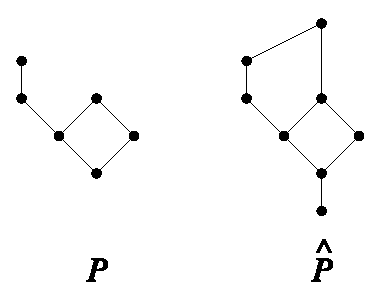
\includegraphics[height=0.2\textheight]{fig/stanley/3-3}
	\caption{\label{fig:stanley:3-3} Adjoining a $\hat{0}$ and $\hat{1}$, from
\citet*{Stanley:2011:ECV:2124415}.}
\end{figure}

We denote by \(\hat{\P}\) the poset obtained from \(\P\) by adjoining a
\(\hat{0}\) and \(\hat{1}\) (in spite of a \(\hat{0}\) or \(\hat{1}\) which
\(\P\) may already possess). In \ref{fig:stanley:3-3} we show an example of
this operation applied to some posets.
